\section{Introduction}

This chapter applies the methods of chapters \ref{chap:dist-opt} and \ref{chap:rect-basis}, specifically algorithms \ref{dadmm_algo_lasso}, \ref{alg:single-slot} and \ref{alg:multiple-shot} to a data set of TVWS measurements captured by OFCOM in the band 440-780MHz. The OFCOM dataset was taken in Southwark, UK during May 2014.

This chapter is organised as follows: we first describe the dataset in detail, and show example PSD captures for it, then we show results of the distributed estimation algorithm (presented in chapter \eqref{chap:dist-opt}), with estimation in the Heavyside basis. This algorithm is performed over a network of nodes, and reconstructs the sensed PSD via an iterative denoising procedure derived from the LASSO functional. It should be noted that this is the largest experiment of its kind: previous work has featured experimental results on far smaller datasets, or featured algorithms whos steps took considerably longer to reach an acceptable solution. We compare results produced by our algorithm to results from copetative algorithms, and discuss the relative performance in terms of reconstruction quality, classification accuracy and algorithm speed. 

We then present results of the techineques outlined in chapter \eqref{chap:cs-inference}, specifically algorithms \ref{alg:single-slot} and \ref{alg:multiple-shot} on the OFCOM data set. These algorithms aim at classifying the signal directly from compressive measurements without reconstructing the signal as an intermediate step. The major feature of these methods is that classification can still be done accurately with sever undersampling. We compare the undersampling capabilities of a single shot algorithm, and one which borrows statistical strength from multiple time slots to reduce the sampling further.

\section{Data Set}

This data set was kindly supplied by OFCOM, and is of the 440-790 MHz TVWS band, with a resolution of 25 kHz. The data was captured at Riverside House, Southwark, London. 

There was no ground truth signal provided with the data set, so so quantitatively asses whether or not out methods are working, we established one by taking the average of several of the captures and then plotting a denoised line by eye. We don't believe that this is an entirely satisfactory option, but the OFCOM frequency allocation doens't give specific enough geographic information to reconstruct a typical PSD. 

\begin{figure}[h]
\centering
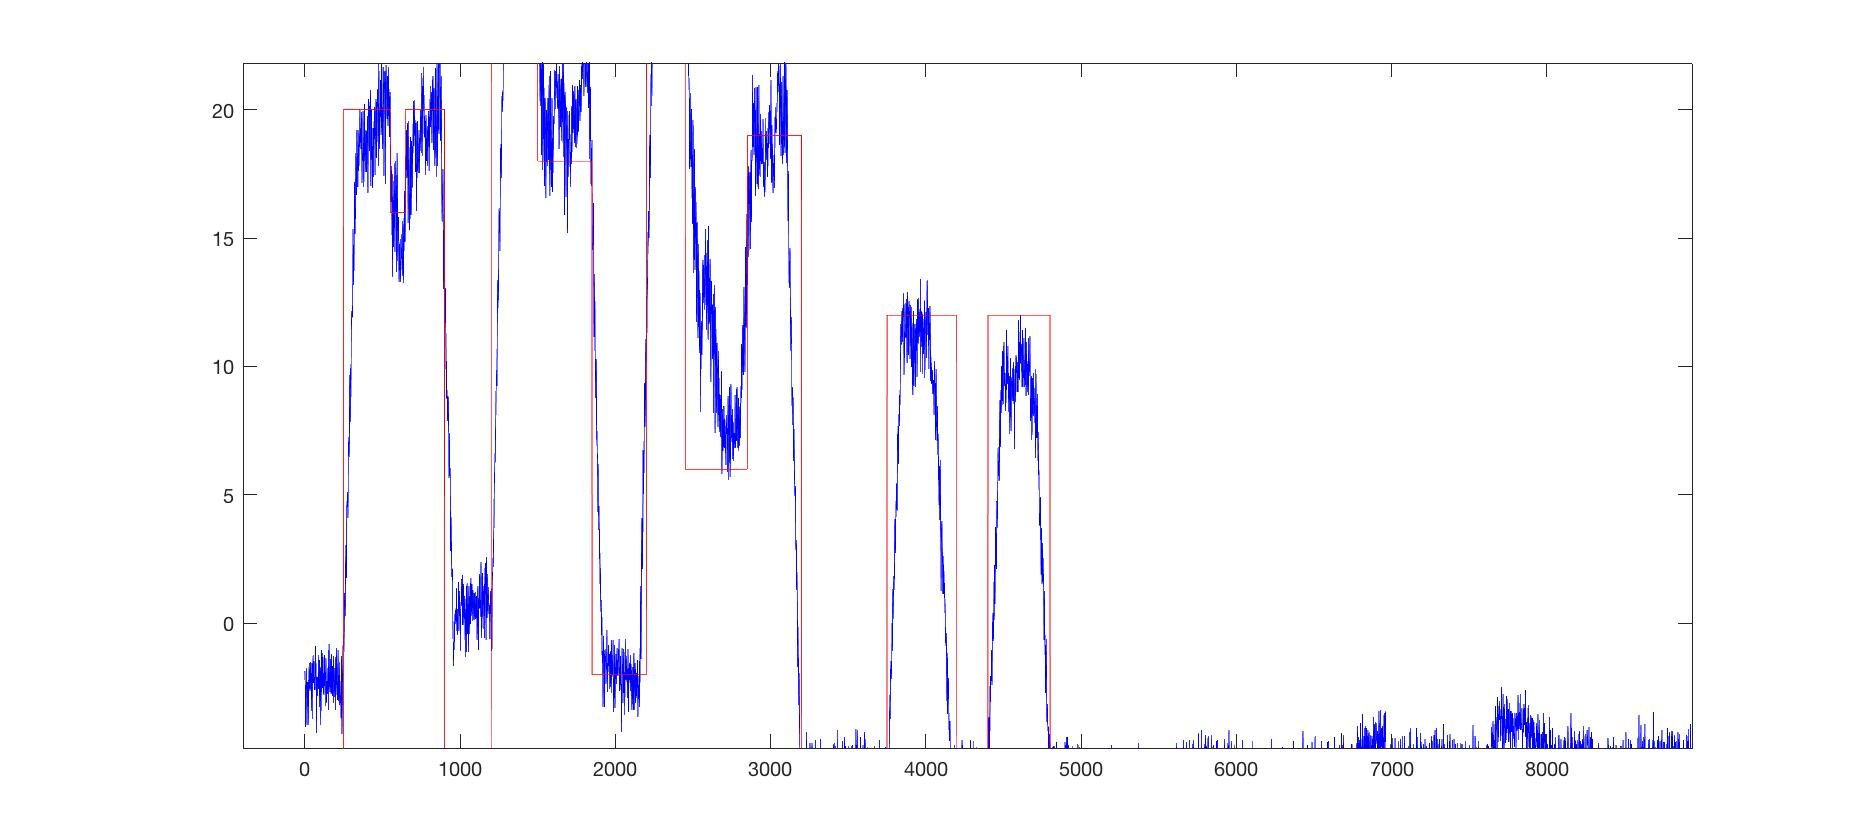
\includegraphics[height = 7.3 cm]{ofcom_ground_truth.jpg}
\caption{}
\label{fig:hvb}
\end{figure}


\section{Results: Distributed Estimation with Heaviside Basis}

\begin{figure}[h]
\centering
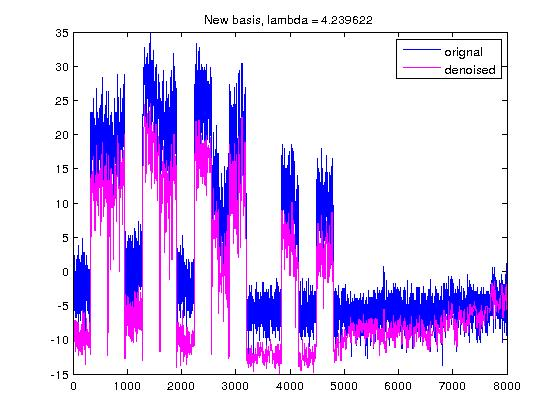
\includegraphics[height = 7.3 cm]{new_basis_ofcom_1.jpg}
\caption{Example of classification with OFCOM data, 35 changepoints}
\label{fig:hvb}
\end{figure}

\begin{figure}[h]
\centering
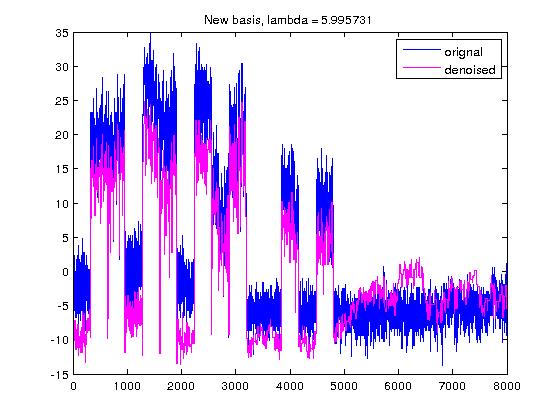
\includegraphics[height = 7.3 cm]{new_basis_ofcom_2.jpg}
\caption{Example of classification with OFCOM data, 55 changepoints}
\label{fig:hvb}
\end{figure}

\begin{figure}[h]
\centering
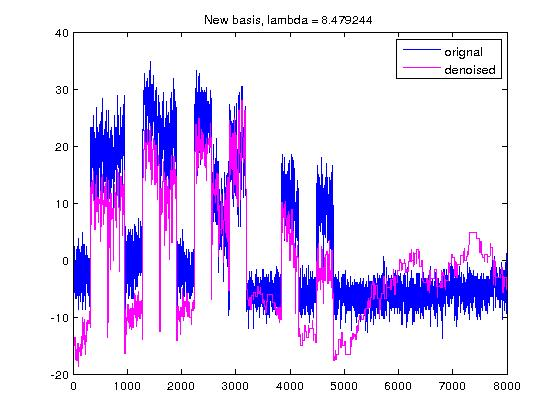
\includegraphics[height = 7.3 cm]{new_basis_ofcom_3.jpg}
\caption{Example of classification with OFCOM data, 35 changepoints}
\label{fig:hvb}
\end{figure}

\begin{figure}[h]
\centering
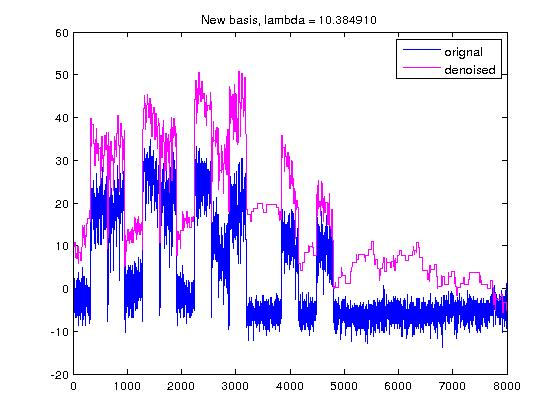
\includegraphics[height = 7.3 cm]{new_basis_ofcom_4.jpg}
\caption{Example of classification with OFCOM data, 55 changepoints}
\label{fig:hvb}
\end{figure}

These figures show that qualitatively, the distributed algorithm is capable of reconstructing the PSD in the TVWS band. This is good as it shows that a distributed algorithm is in principle capable of performing a large-scale reconstruction of PSD. It should be noted that to our knowledge, this is the only study using data sets this size. 

All these plots show significant co-linearlity between samples, so to address this we tried a distributed version of the Elastic Net. 

To more quantitatively asses how well our algorithm perfromed we...

\section{Compressive Estimation}

Some examples of the output of procedure \ref{alg:single-shot} are shown below, as applied to the OFCOM data set.

\begin{figure}[h]
\centering
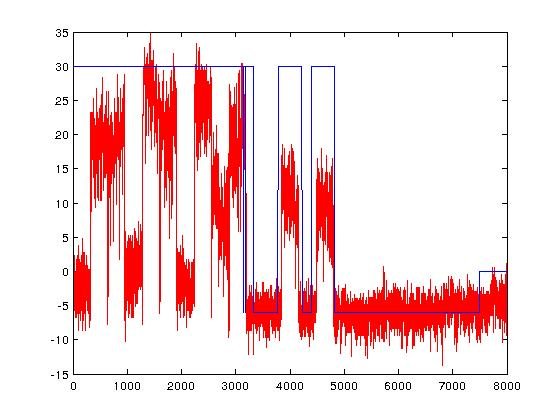
\includegraphics[height = 7.3 cm]{ofcom_classification1.jpg}
\caption{Example of classification with OFCOM data, 35 changepoints}
\label{fig:hvb}
\end{figure}

\begin{figure}[h]
\centering
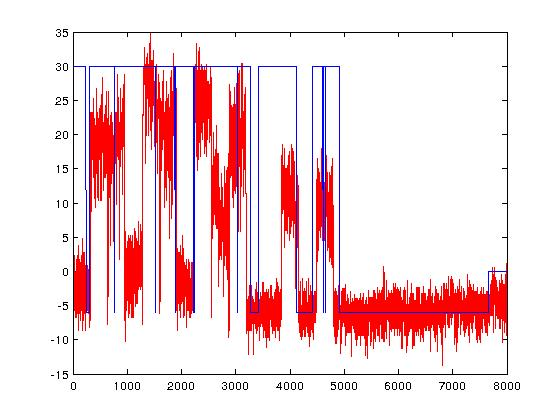
\includegraphics[height = 7.3 cm]{ofcom_classification.jpg}
\caption{Example of classification with OFCOM data, 55 changepoints}
\label{fig:hvb}
\end{figure}

\begin{figure}[h]
\centering
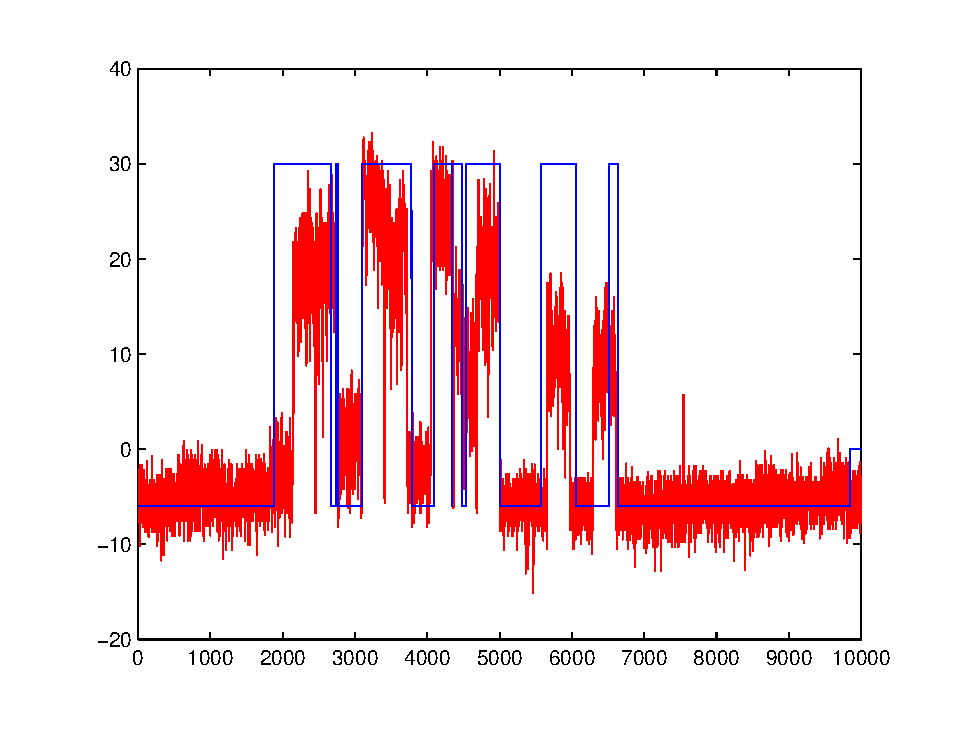
\includegraphics[height = 7.3 cm]{OFCOM5.eps}
\caption{Example of classification with OFCOM data, 35 changepoints}
\label{fig:hvb}
\end{figure}

\begin{figure}[h]
\centering
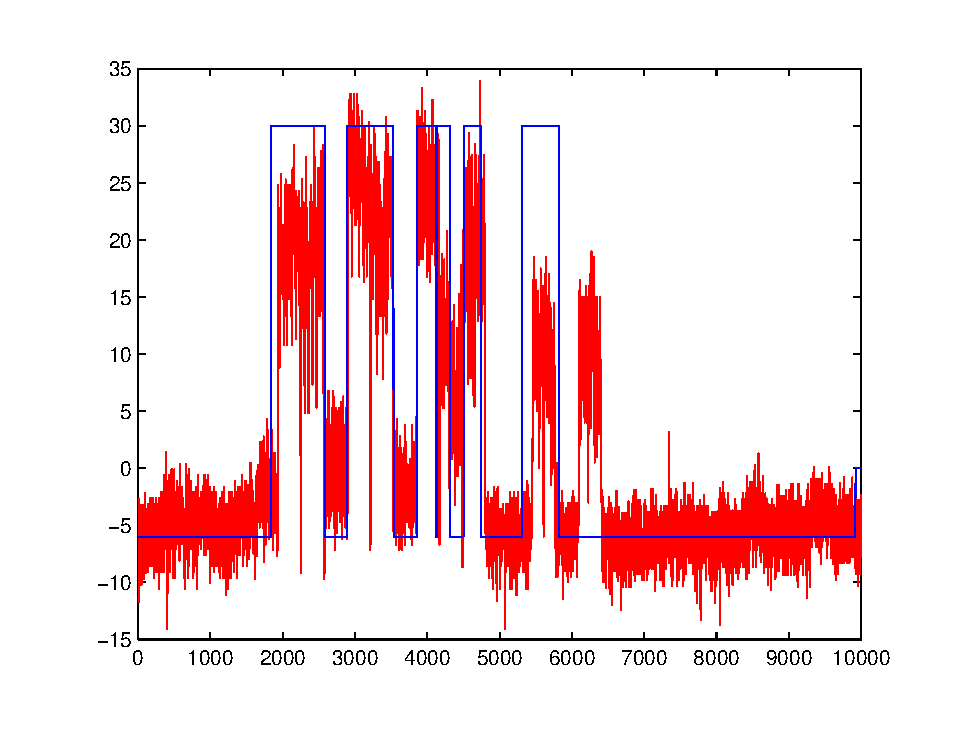
\includegraphics[height = 7.3 cm]{OFCOM6.eps}
\caption{Example of classification with OFCOM data, 55 changepoints}
\label{fig:hvb}
\end{figure}

\begin{figure}[h]
\centering
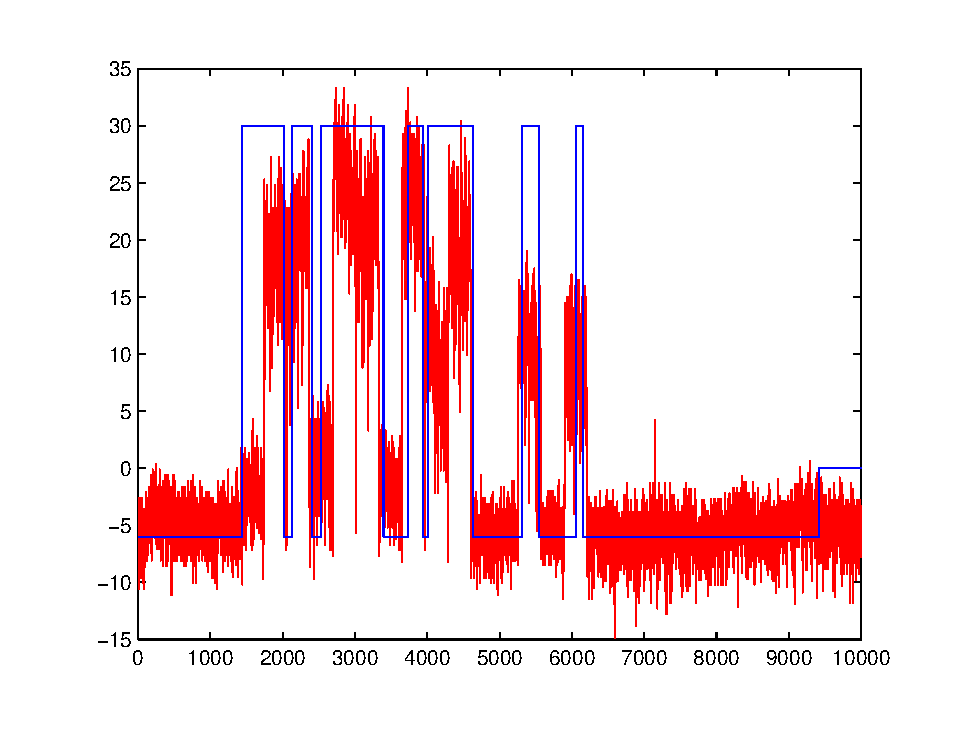
\includegraphics[height = 7.3 cm]{OFCOM7.eps}
\caption{Example of classification with OFCOM data, 35 changepoints}
\label{fig:hvb}
\end{figure}

\begin{figure}[h]
\centering
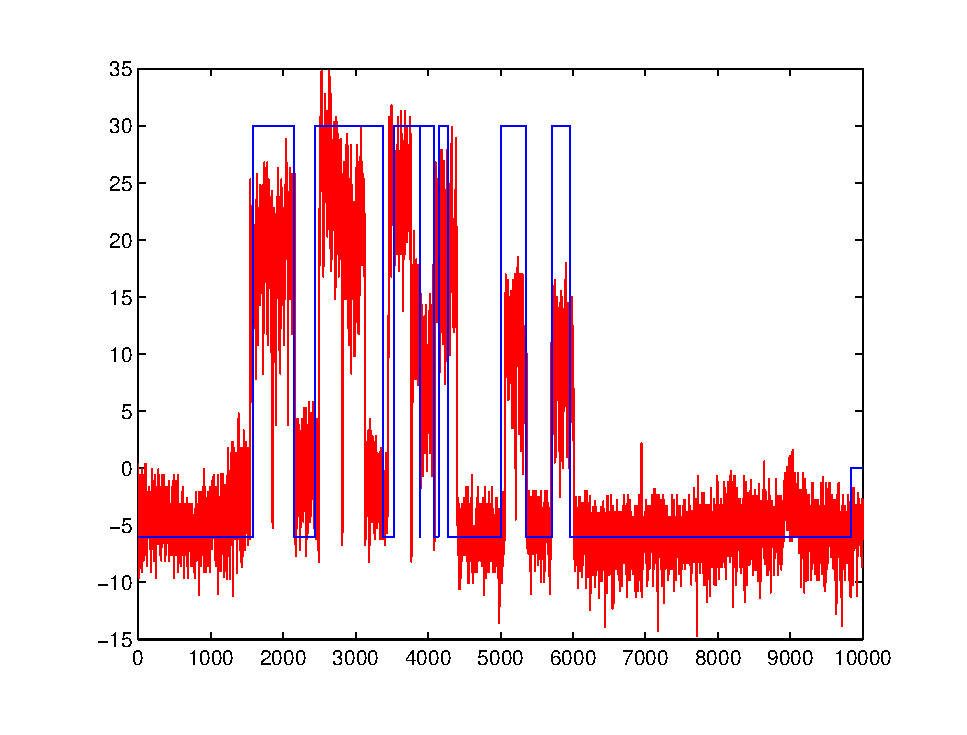
\includegraphics[height = 7.3 cm]{OFCOM8.eps}
\caption{Example of classification with OFCOM data, 55 changepoints}
\label{fig:hvb}
\end{figure}

\section{Conclusions}